\subsection{Political Differences}\label{sec_res_exp}

    \paragraph{Labeled Subsample Characteristics}

    Table \ref{tab_corp_charac_subs} presents simple textual statistics for the subsample of the main corpus labeled by political affiliation. Appendix Figures \ref{random_tweets_lef} and \ref{random_tweets_rig} show four random tweets from left-leaning and right-leaning Twitter users, respectively. Given that Twitter data generally is biased (as discussed in Section \ref{sec_lit}), and our labeling strategy is rather simple (see Steps 6-7 in Section \ref{sec_meth_gene}), the subsample of left- and right-leaning Twitter users might be more biased than the main corpus, over-representing more extreme positions. However, the results presented in this section are still consistent with previous studies, as is further discussed in Section \ref{sec_disc_prev}.

    \begin{table}[H]
            %\footnotesize
            \centering
            
            \subfile{tabs/corp_charac_subs}
            
            \caption{Corpus Characteristics, Political Affiliation-Labeled Subcorpus}
            
            \floatfoot{\it 
            Notes: Unique words and hashtags can have duplicates across the subcategories ''left-leaning'', ''right-leaning'' or ''unlabeled''.
            \vspace{0.5em} \\
                    Data Source: Retrieved from Twitter API, spanning the time frame Nov 1\textsuperscript{st}, 2020 -- April 11\textsuperscript{th}, 2022. Corpus includes tweets by Twitter users in Chile or Chilean nationals that mainly pertain to immigration. Corpus cleaned by the steps in our methodology as described in Section \ref{sec_meth_gene} and Appendix \ref{app_sec_meth}.}
            \label{tab_corp_charac_subs}
        \end{table}
        
    From Table \ref{tab_corp_charac_subs}, it is seen that the number of left-leaning and right-leaning labeled Twitter users is approximately balanced. However, right-leaning Twitter users tweet almost thrice as much as left-leaning users in the given time frame. Right-leaning users are responsible for 27.4\% of total tweets compared to only 10.3\% from left-leaning users. We also find that right-leaning users post on average 31 tweets while left-leaning users post 13 tweets on average. So, it holds that right-leaning Chilean Twitter users are significantly more active regarding immigration than left-leaning users despite the almost equal number of left-leaning and right-leaning Twitter users.\footnote{It is difficult to interpret results from the 'Unlabeled' category as this possibly includes center-leaning or ideologically neutral users (such as media outlets), or uncategorized right- and left-leaning users that our classification strategy does not classify. Some of our results, however, seem to indicate that this category mainly consists of right-leaning Twitter users. These findings are presented in Section \ref{unlab_users_affiliation}. A relevant future improvement for our research is to utilize more accurate methods to label Twitter users by ideology as is discussed further in Section \ref{sec_disc_improv}.} 
    We find further support for this using networks metrics in Section \ref{sec_res_nets}, which also shows that right-leaning Twitter users are more influential and interconnected regarding the topic of immigration than left-leaning users.
    
    
    \paragraph{Sentiments over Time by Ideology}
    
    To extend on the findings from Section \ref{sec_res_corp}, that Chilean Twitter users generally have become more anti-immigration over time, while some highlight anti-xenophobia agendas, we extend Figure \ref{fig_words_over_time} by distinguishing Twitter users by political affiliation. Figure \ref{fig_terms} presents the percentage of tweets per day that contain terms related to either illegal immigration, crime and xenophobia by political affiliation.
    
    
\begin{figure}[H]
    \caption{Proportion of Tweets Containing Specific Subtopic-Related Terms by Political Affiliation during the Protest; Sep 21, 2021 -- Oct 1, 2021}
    \label{fig_terms}
    
    \centering
        \begin{subfigure}{0.5\textwidth}
            %\caption{Anti-Xenophobia-Related}
            \centering
            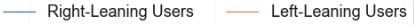
\includegraphics[width=.85\linewidth]{figs/Comparison_Legend.jpg}
            %\label{fig_xenophobia_terms}
        \end{subfigure}
    \hfill
        \begin{subfigure}{0.5\textwidth}
            \caption{Illegal Immigration-Related Terms}
            \centering
            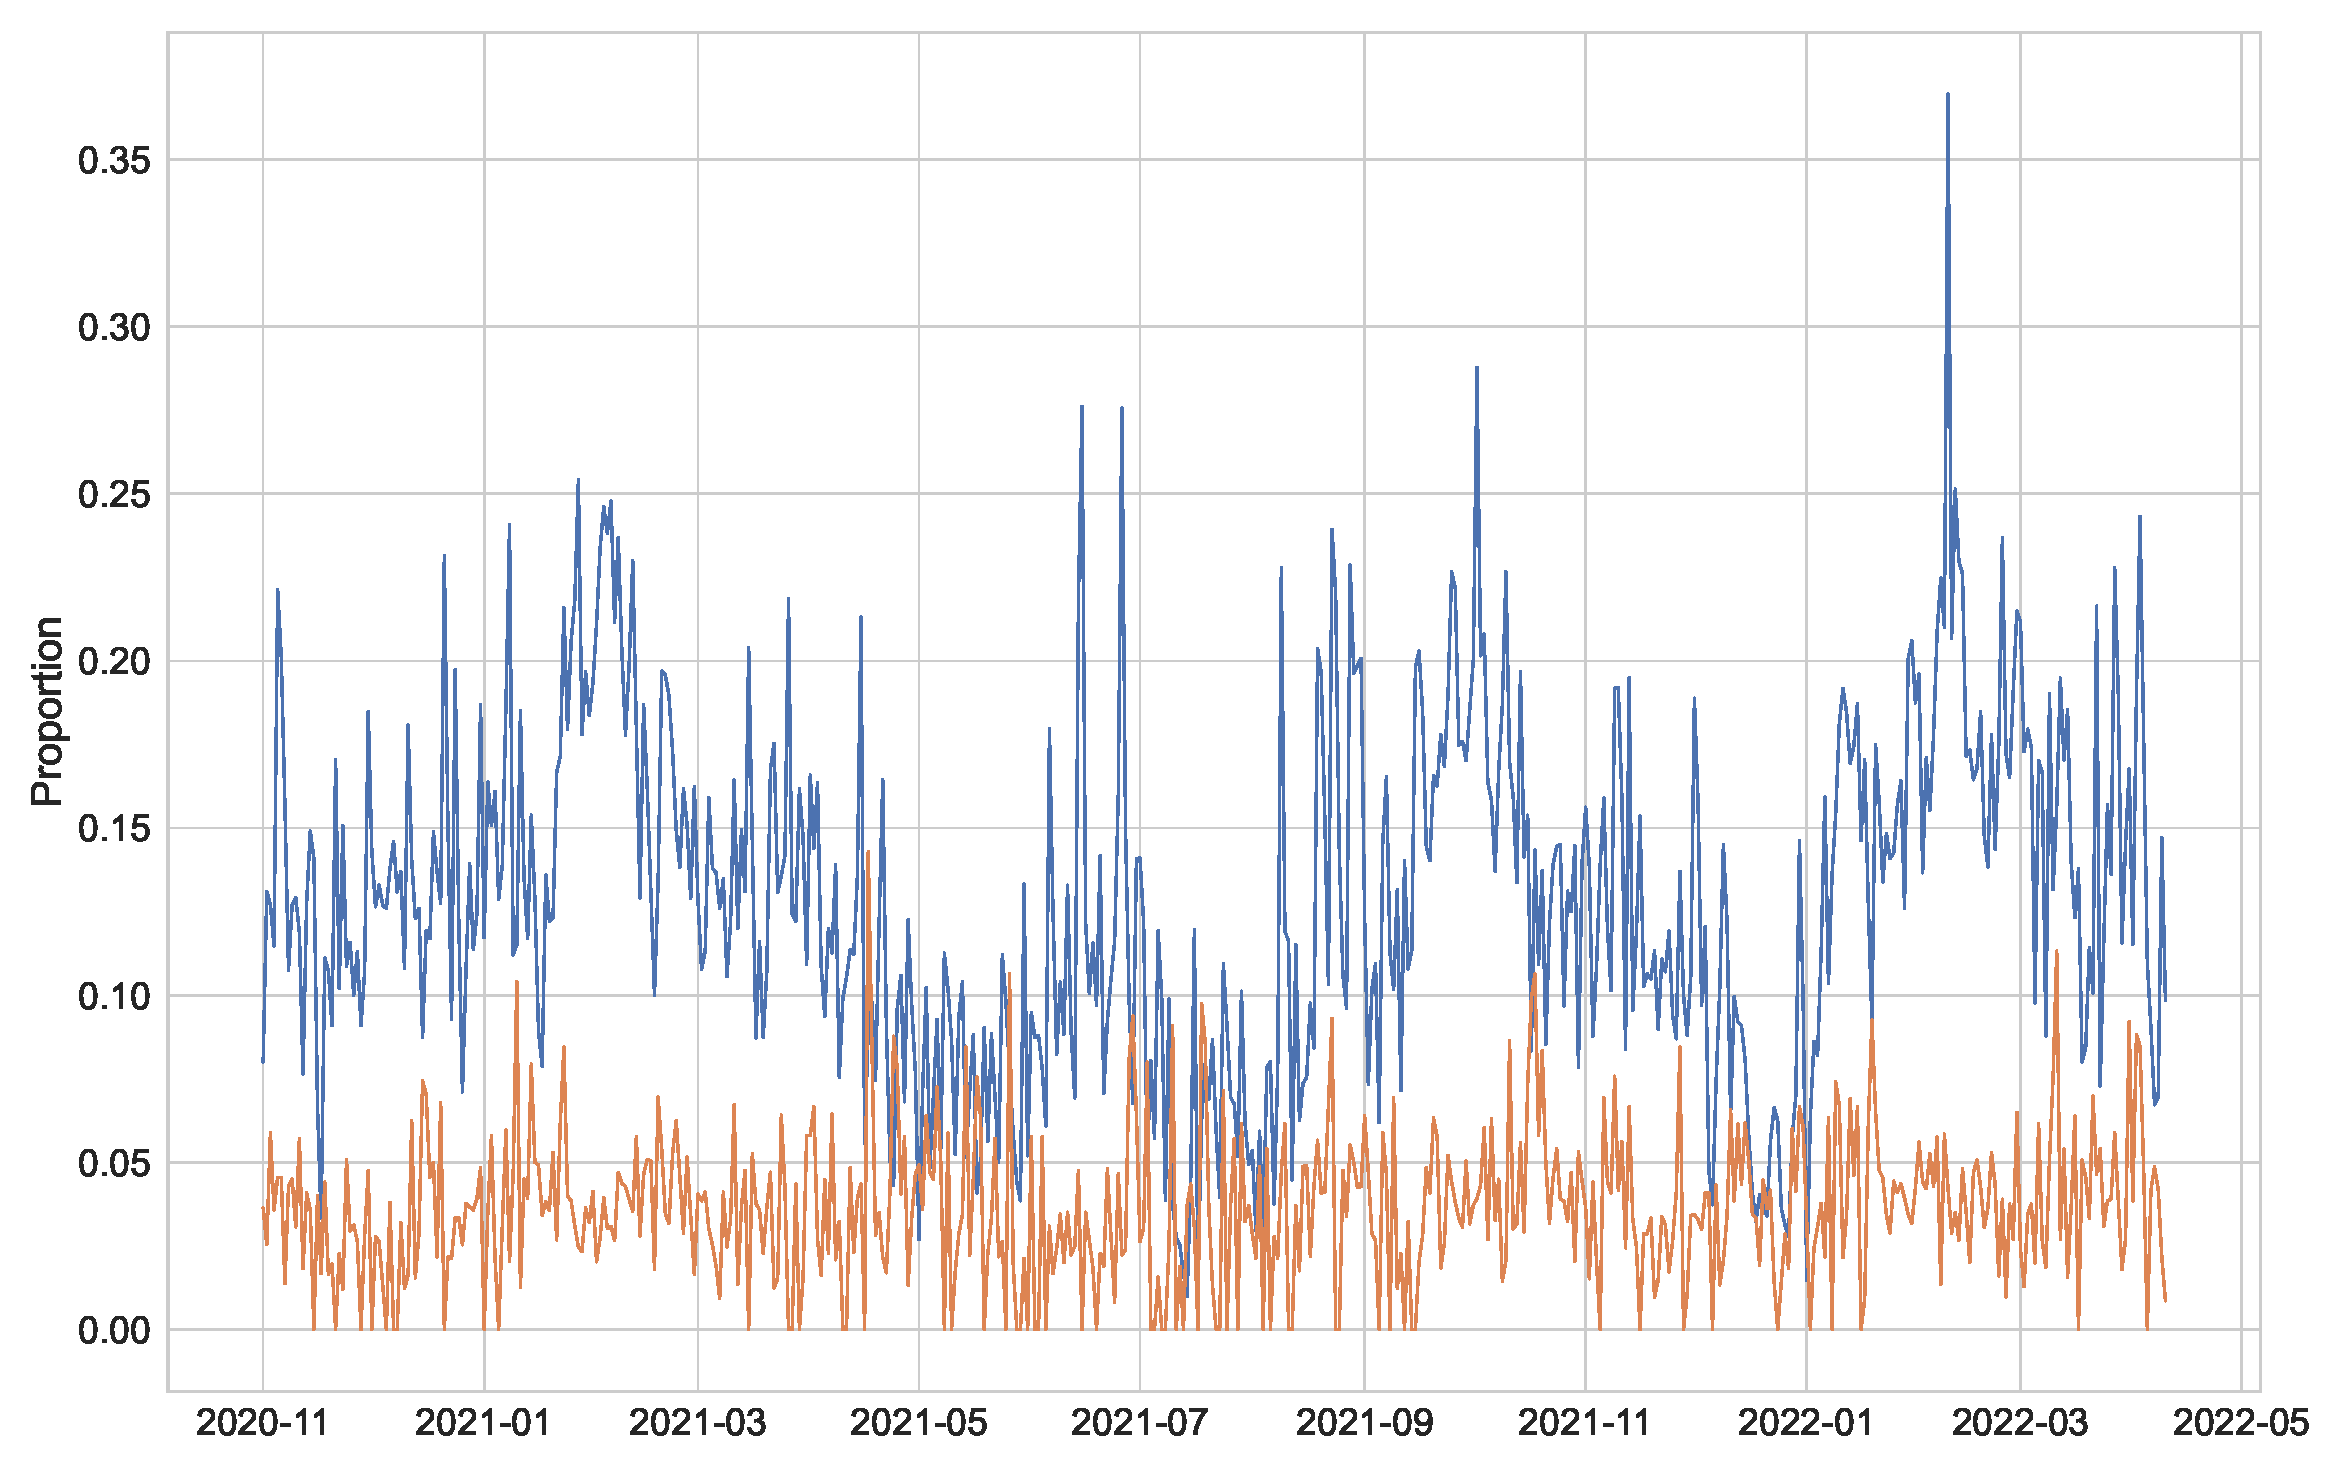
\includegraphics[width=.99\linewidth]{figs/Comparison_illegal_terms.eps}
            \label{fig_irregular_terms}
        \end{subfigure}%
    %\hfill
        \begin{subfigure}{0.5\textwidth}
            \caption{Crime-Related Terms}
            \centering
            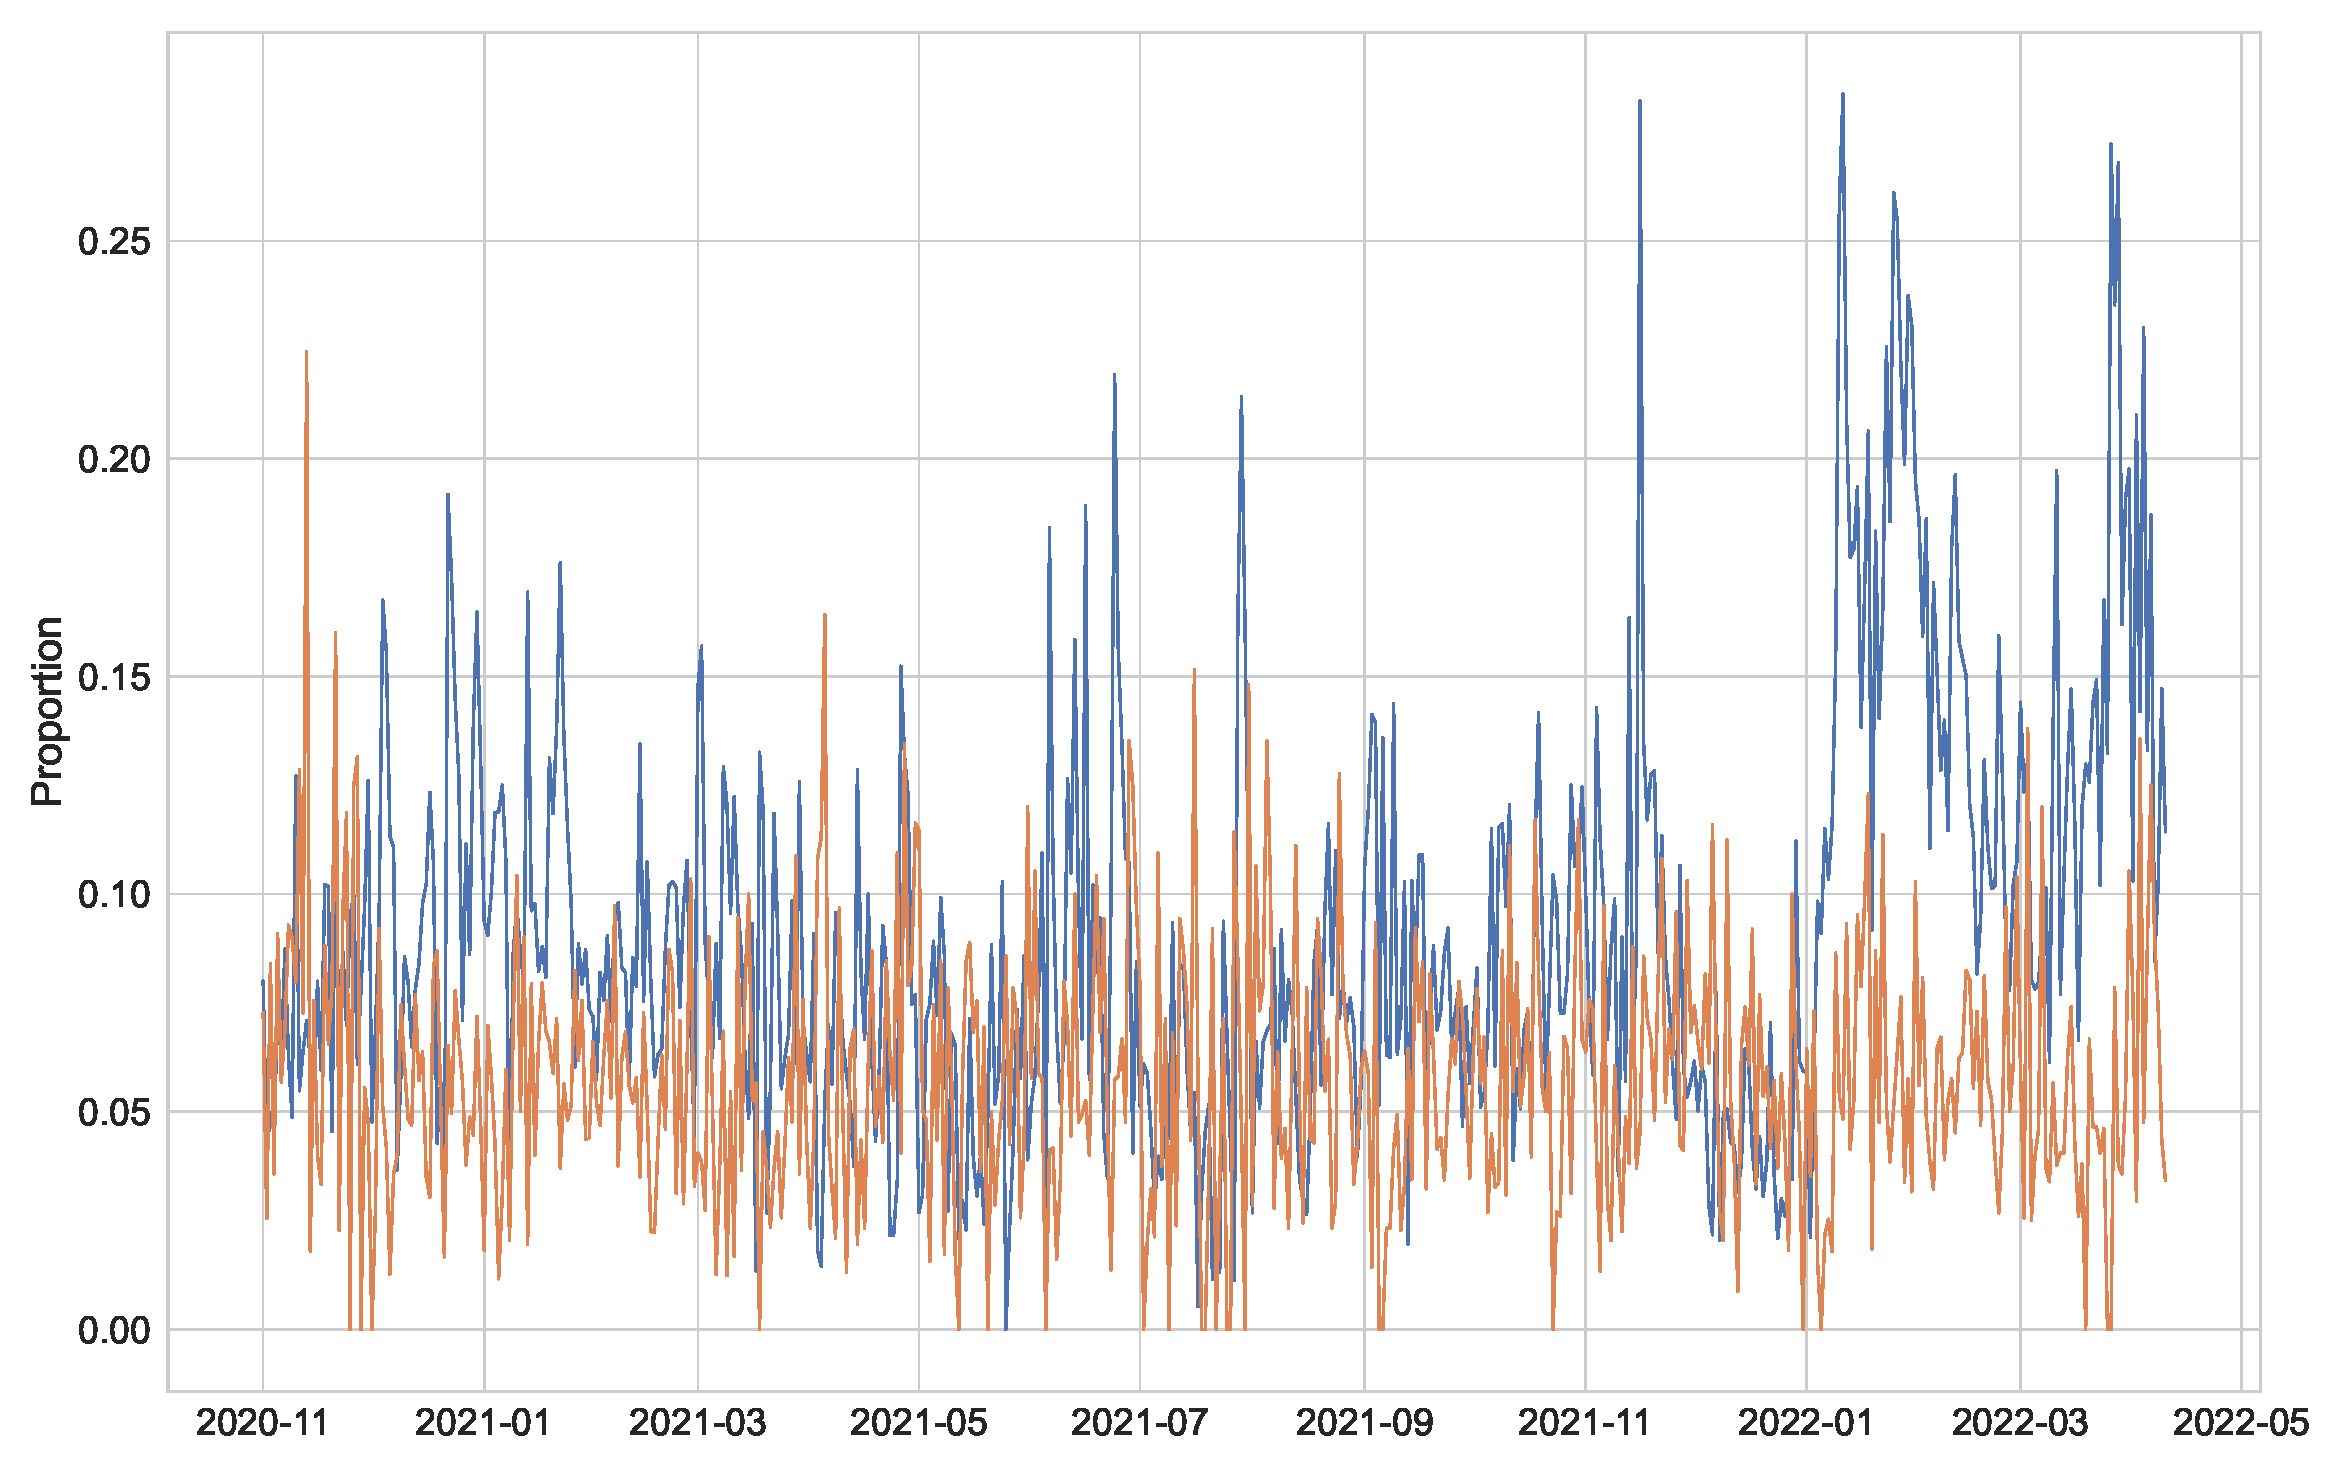
\includegraphics[width=.99\linewidth]{figs/Comparison_Crime_terms.eps}
            \label{fig_crime_terms}
        \end{subfigure}
    \hfill
        \begin{subfigure}{0.5\textwidth}
            \caption{Anti-Xenophobia-Related Terms}
            \centering
            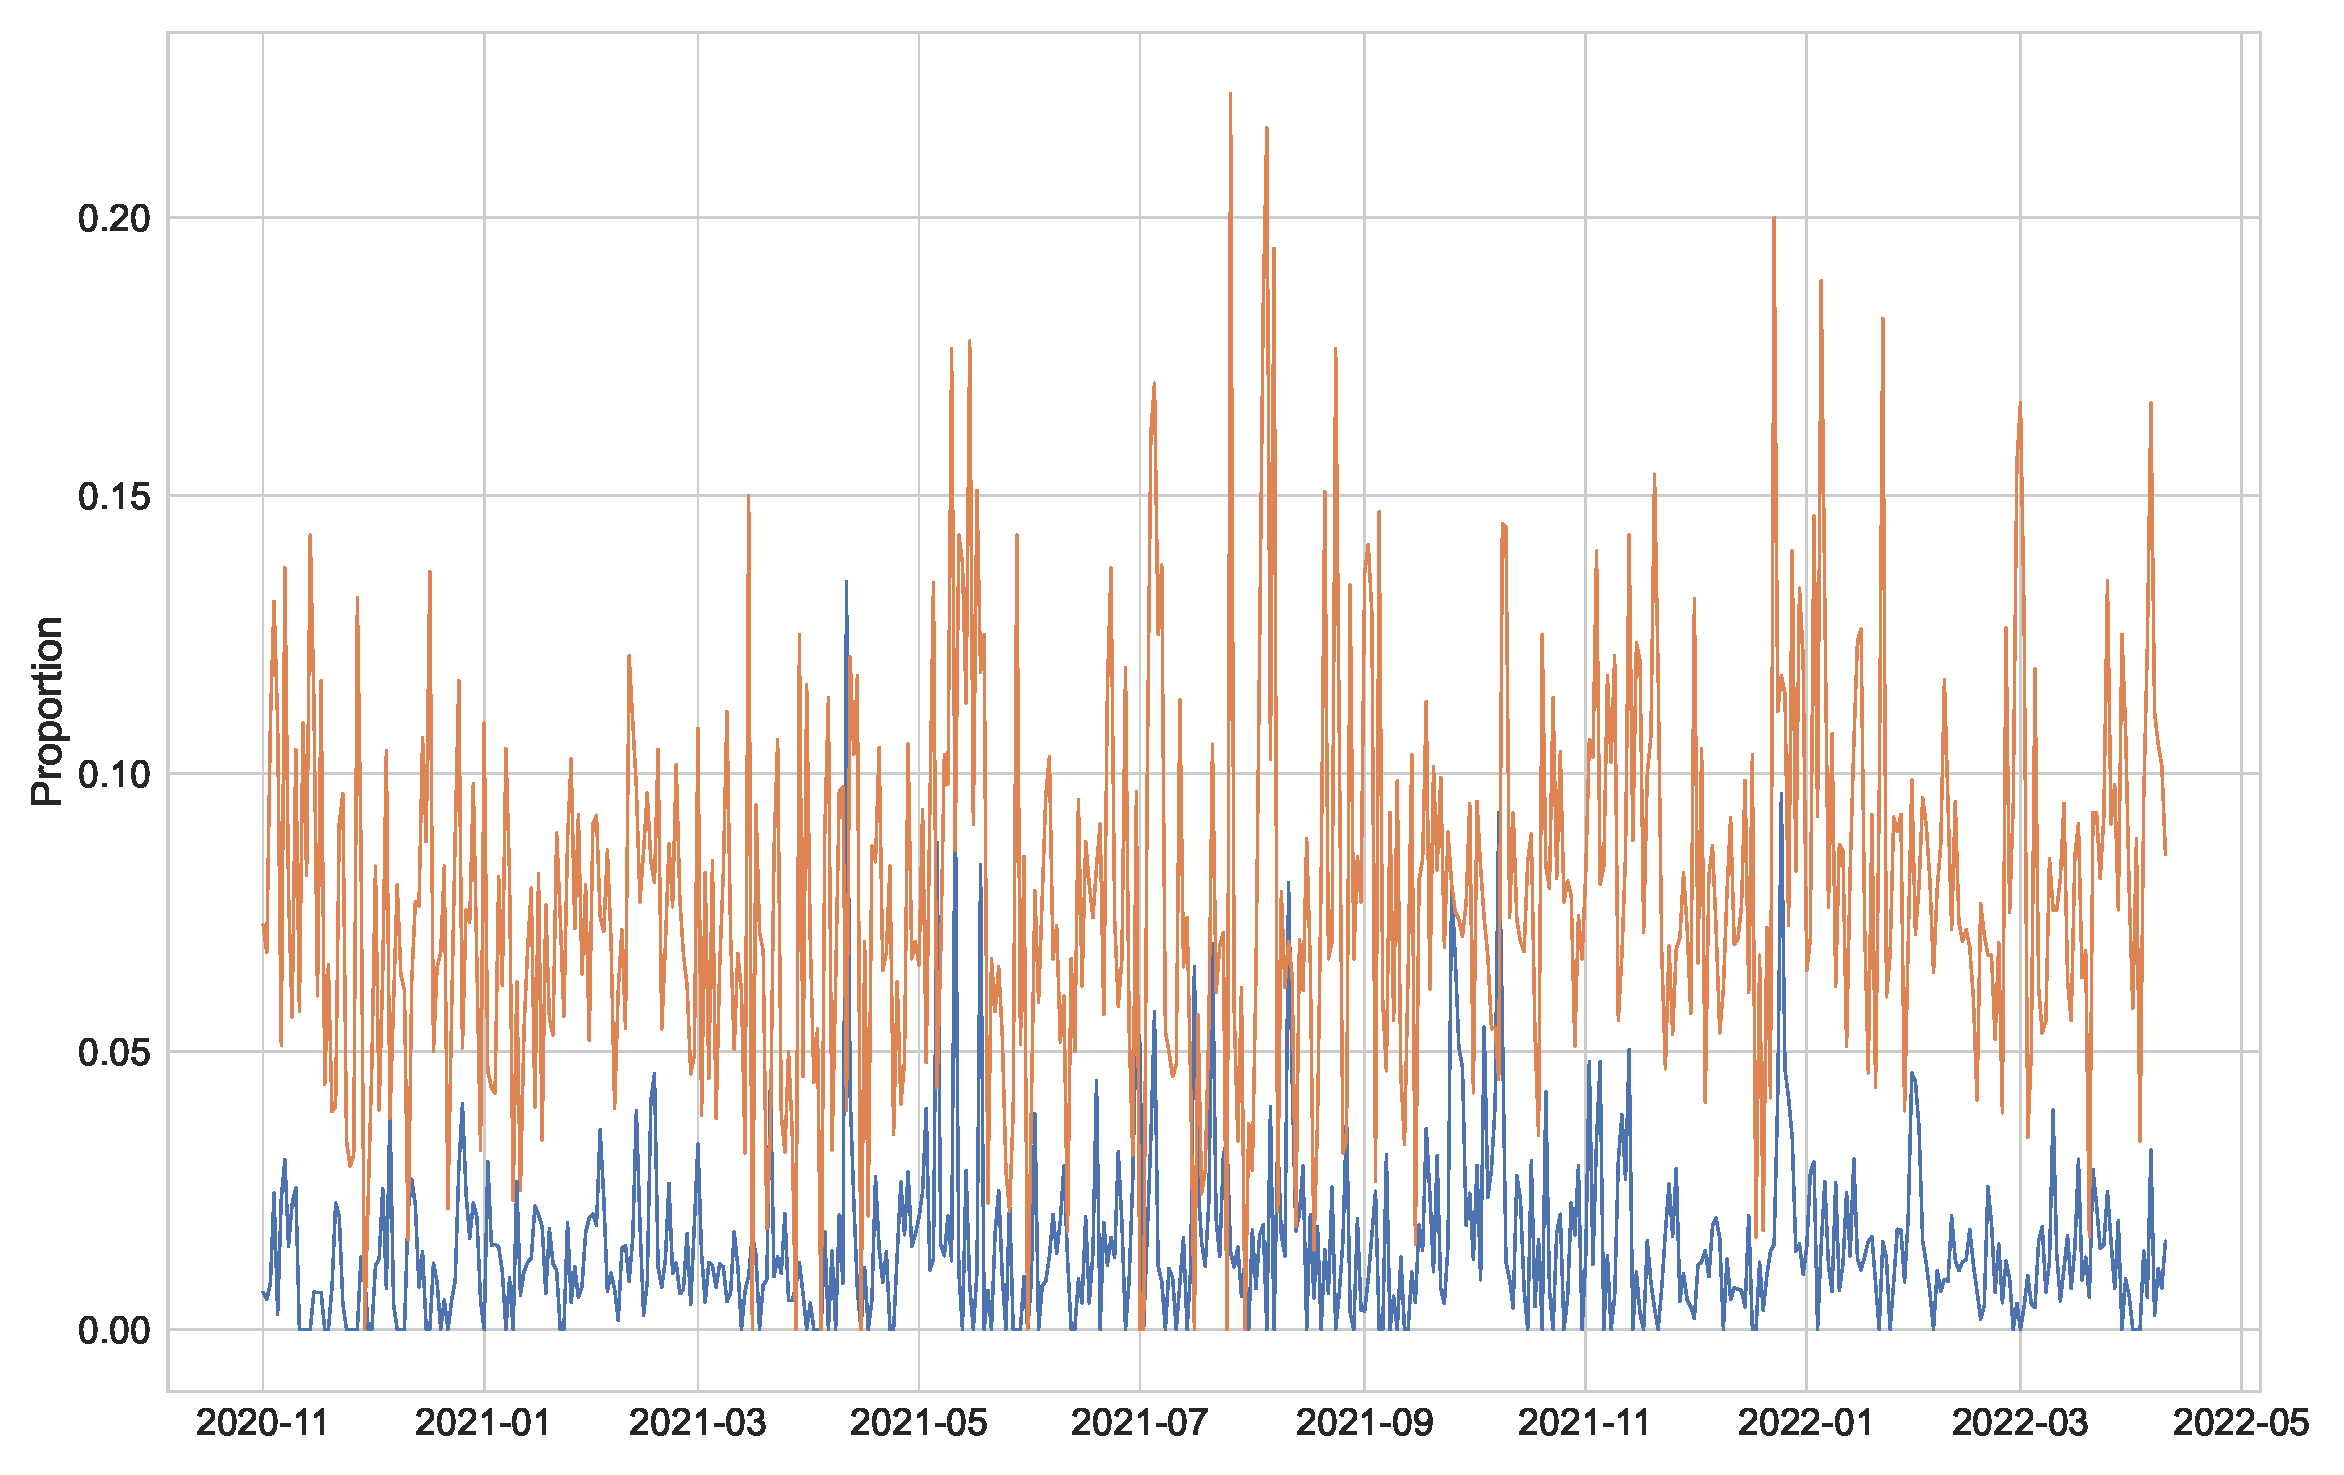
\includegraphics[width=.99\linewidth]{figs/Comparison_Xenophbia_terms.eps}
            \label{fig_xenophobia_terms}
        \end{subfigure}
    %\hfill
    
    \floatfoot{\it 
        Notes: Orange line is for left-leaning Twitter users and blue is for right-leaning ones. Tweets in each of the subfigures are filtered by whether they contain at least one term in a specified list of terms. List of terms in Figure \ref{fig_irregular_terms}: {\it 'ilegal'}, {\it 'ilegales'}, {\it 'indocumentado'}, {\it 'indocumentados'}. List of terms in Figure \ref{fig_crime_terms}: {\it 'delincuentes'}, {\it 'delincuencia'} , {\it 'crimen'}, {\it 'criminiales'}, {\it 'delito'}, {\it 'delitos'}, {\it 'robo'}, {\it 'ladron'}, {\it 'ladrones'}. List of terms in Figure \ref{fig_xenophobia_terms}: {\it 'xenofobia'}, {\it 'racismo'}, {\it 'discriminacion'}, {\it 'discriminados'}. Textual preprocessing steps in outputs include lowercase enforcement and converting Spanish special characters (e.g. á, ñ, etc.) into corresponding non-accentuated ones.
        \vspace{0.5em} \\
        Data Source: Subsample of main corpus retrieved from Twitter API, spanning the time frame Nov 1\textsuperscript{st}, 2020 -- April 11\textsuperscript{th}, 2022. Affiliation labels constructed using Step 6 in our methodology as described in Section \ref{sec_meth_gene} and Appendix \ref{app_sec_meth}. Corpus includes tweets by Twitter users in Chile or Chilean nationals that mainly pertain to immigration.}
\end{figure}

    From Figure \ref{fig_irregular_terms} it is seen that terms regarding illegal immigration are mostly used by right-leaning users while terms related to anti-xenophobic agendas are mostly used by left-leaning users (Figure \ref{fig_xenophobia_terms}). With few exceptions these trends are approximately constant across the considered time frame. This finding is consistent with what could be hypothesized for each political affiliation. Surprisingly, the use of crime-related terms gives a more ambiguous picture as shown in Figure \ref{fig_crime_terms}. Until the beginning of 2022, crime-related terms are used in approximately equal proportions between right-leaning and left-leaning users. However, since the beginning of 2022 (following the presidential election), right-leaning users begin to increase their usage of crime-related terms. This might explain the findings in Figure \ref{fig_words_over_time} where the usage of the term {\it 'delincuentes'} begins to overtake {\it 'ilegales'} in the latter period.  The increase in usage of crime-related terms by right-leaning users coincides with the third peak in Twitter activity after the anti-immigration protests in February 2022. Contrary to general Twitter activity following the peak (see Figure \ref{total_tweets_per_day}), the proportion of crime-related terms in Figure \ref{fig_crime_terms} does not diminish after the protest. This might indicate that right-leaning users begin to push agendas equating immigration with crime few weeks after the new leftist government was elected in December 2021.


    \paragraph{Analysis of a Specific Event}
    Governments might be interested in analyzing what is happening in the Twittersphere during unusually high peaks of activity. The highest peak of activity in our corpus occurred in September 2021 coinciding with violent anti-immigration protest in the northern border city of Iquique, as mentioned in Section \ref{sec_res_corp}. For the sake of this analysis, we consider 5 days before and 5 days after the protest, i.e. September 21\textsuperscript{st}, 2022 to October 1\textsuperscript{st}, 2022. 
    
    Figure \ref{fig_bigram_protest} presents the most-used bigrams during the protest period for left- and right-leaning Twitter users, respectively (Figure \ref{fig_bigram_protest_lef} and \ref{fig_bigram_protest_rig}, respectively). The figure shows that right-leaning Twitter users put their main emphasis on illegal immigration during the protest. Left-leaning users use a more uniformly distributed collection of bigrams, but a large part of them seem to indicate more embracing and guestfriendly views towards migrants. This is exemplified by bigrams such as {\it 'invito, venezolanos'} (Eng: Invited, Venezuelans) and {\it 'venezolanos, venir'} (Eng: Venezuelans, come). We also find anti-xenophobic sentiments such as {\it 'xenofobia, racismo'} (Eng: Xenophobia, racism) and sympathies towards the immigrants' destroyed belongings by the protesters, e.g. {\it 'pertenencias, migrants'} (Eng: Belongings, immigrants) and {\it 'coches, pañales} (Eng: cars, diapers).\footnote{During the most violent episodes of the protests, the protesters burned many of the immigrants belongings such as tents and diapers.}
    
    \begin{figure}[H]
        \caption{Top 15 Bigrams for Twitter Users during the Protest; Sep 21, 2021 -- Oct 1, 2021}
        \label{fig_bigram_protest}
        
        \centering
            \begin{subfigure}{0.5\textwidth}
                \caption{Left-Leaning Twitter Users}
                \centering
                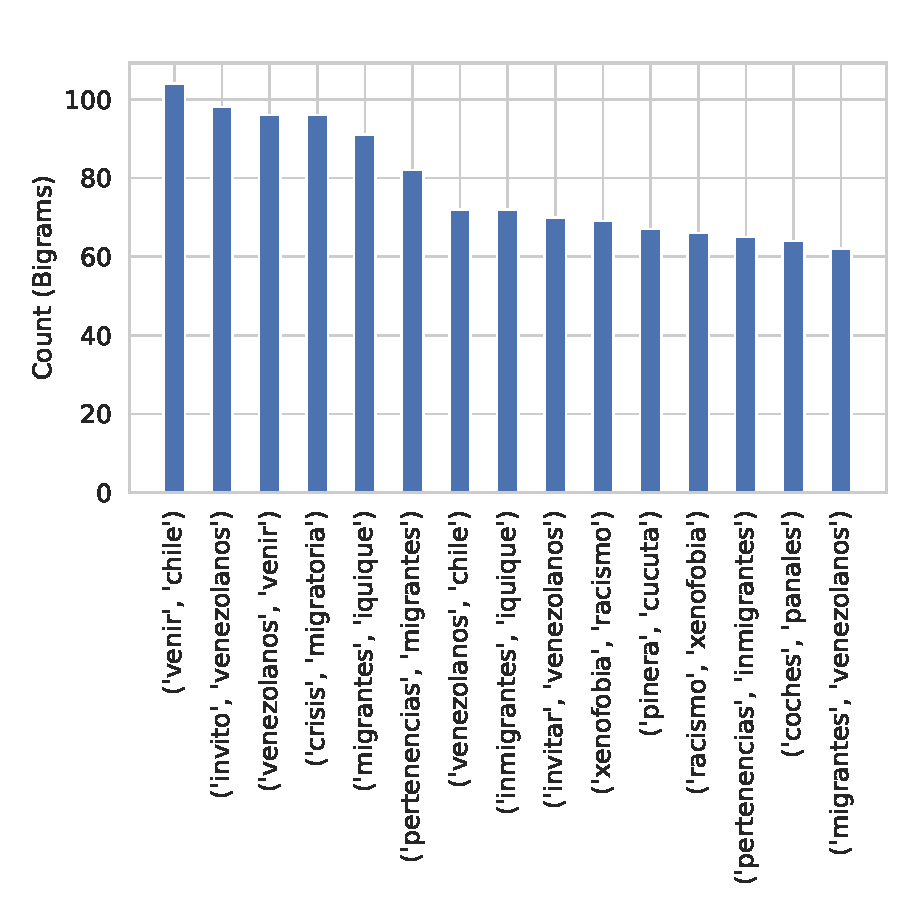
\includegraphics[width=.99\linewidth]{figs/Left_Bigrams_Protest_1.eps}
                \label{fig_bigram_protest_lef}
            \end{subfigure}%
        %\hfill
            \begin{subfigure}{0.5\textwidth}
                \caption{Right-Leaning Twitter Users}
                \centering
                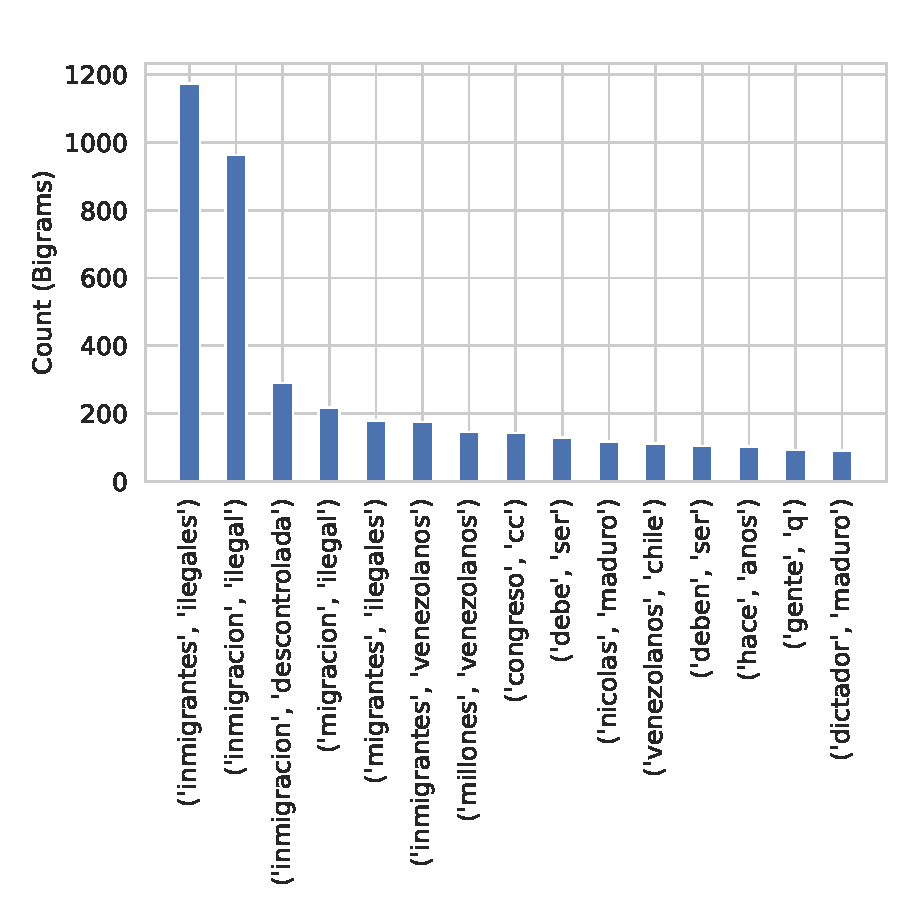
\includegraphics[width=.99\linewidth]{figs/Right_Bigrams_Protest_1.eps}
                \label{fig_bigram_protest_rig}
            \end{subfigure}
        \hfill
            \begin{subfigure}{0.7\textwidth}
                \caption{Unlabeled Twitter Users}
                \centering
                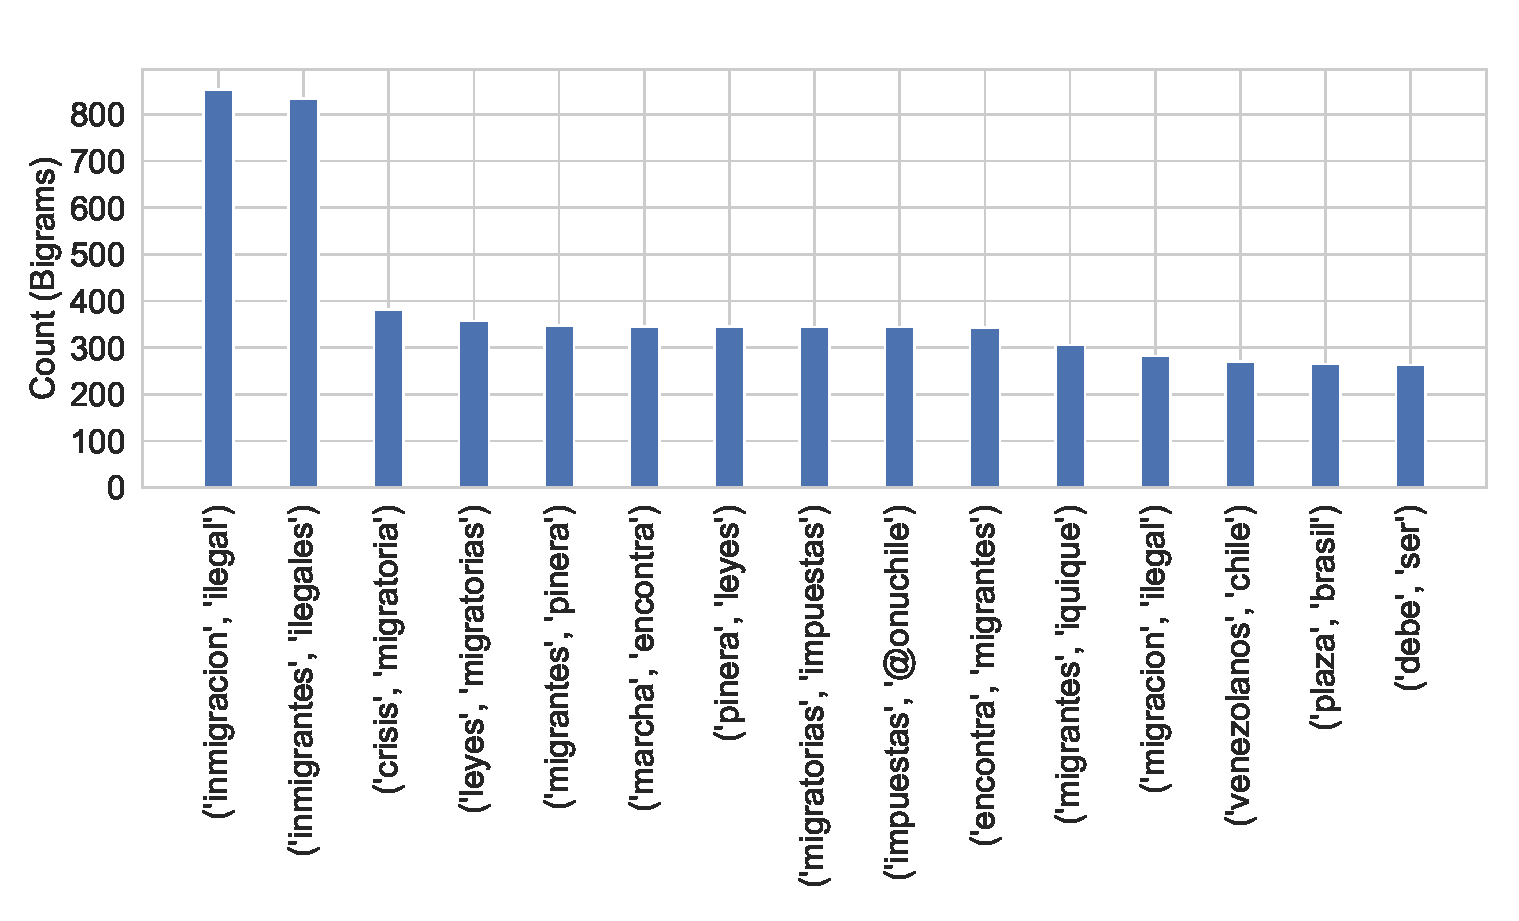
\includegraphics[width=.99\linewidth]{figs/Unlabeled_Bigrams_Protest_wh_1.eps}
                \label{fig_bigram_protest_unlab}
            \end{subfigure}
    
    %kal_bi_unlabeled_protest_1.png
        
    \floatfoot{\it 
                Notes:  Textual preprocessing steps in outputs include lowercase enforcement and converting Spanish special characters (e.g. á, ñ, etc.) into corresponding non-accentuated ones.
                \vspace{0.5em} \\
                Data Source: Subsample of main corpus retrieved from Twitter API, 5 days before and after the protest, i.e. Sep 21, 2021 to Oct 1, 2021. Affiliation labels constructed using Step 6 in our methodology as described in Section \ref{sec_meth_gene} and Appendix \ref{app_sec_meth}. Corpus includes tweets by Twitter users in Chile or Chilean nationals that mainly pertain to immigration.}
    \end{figure}
    
    Comparing these findings with the most-used hashtags by left- and right-leaning users in Figure \ref{fig_hashtags_protest} indicates further support for these findings. For left-leaning users' most popular hashtags in Figure \ref{fig_hashtags_protest_lef}, we again find anti-xenophobia agendas exemplified by hashtags such as \texttt{\#xenofobia} (Eng: Xenophobia), \texttt{\#racismo} (Eng: Racism) and \texttt{\#iquiquemedasverguenza} (Eng: Iquique you embarass me). For the right-leaning users we find further support that these hold strong anti-immigration views in Figure \ref{fig_hashtags_protest_rig}, as seen from the use of hashtags such as \texttt{\#nomasimmigrantes} (Eng: No more immigrants) and \texttt{\#iquiquedicebasta} (Eng: Iquique says stop). We also find the previous focus on undocumented immigration from hashstags such as \texttt{\#nomasimmigrantesilegals} (Eng: No more illegal immigrants). From both sides we find opposition to the opposite side of the ideological spectrum: Left-leaning users utilize \texttt{\#elpeorgobiernodelahistoria} (Eng: Worst government in history\footnote{Referring to the previous right-wing government.}), right-leaning users tweet using \texttt{\#izquierdamiserable} (Eng: Miserable left). An interesting difference between left- and right-leaning users however is that the right-leaning presidential candidate José Kast is endorsed during the protests by his supporters (with hashtags such as \texttt{\#atraveteconkast} (Eng: Go with Kast) and \texttt{\#kastpresidente} (Eng: President Kast)) which is not the case for left-leaning users.%This could explain our finding in Section \ref{sec_res_nets} about the relevance that Kast has in the network and it could be seen as a policy lesson showing a way to increase the relevance of some users taking advantage of some commented event.
    \footnote{
    To distinguish if the popular hashtags and bigrams are prominent because the number of users that include it in their tweets increases or as a result of few users pushing these, Appendix Tables \ref{apptab_left_bigrams_protest} and \ref{apptab_right_bigrams_protest} present the count of users using the 15 top hashtags for left- and right-leaning users, respectively. Appendix Tables \ref{apptab_left_hashtags_protest} and \ref{apptab_right_hashtags_protest} present the top 15 bigrams by political affiliation.
    We observe that in general for left- and right-leaning users, the top hashtags and bigrams represent expressions used by a high number of users. The only exception for left-leaning users is the bigram {\it 'coches, pañales'} that makes reference to burned belongings of immigrants. For right-leaning users the exception is {\it 'congreso, cc'} which is related with political institutions (Congress and Constitutional Convention). In the case of unlabeled users appear more terms used only for a few users, mainly related with UN, migration laws and the previous right-wing President.
    }
    
    \begin{figure}[H]
        \caption{Top 15 Hashtags for Twitter Users during the Protest; Sep 21, 2021 -- Oct 1, 2021}
        \label{fig_hashtags_protest}
        
        \centering
            \begin{subfigure}{0.5\textwidth}
                \caption{Left-Leaning Twitter Users}
                \centering
                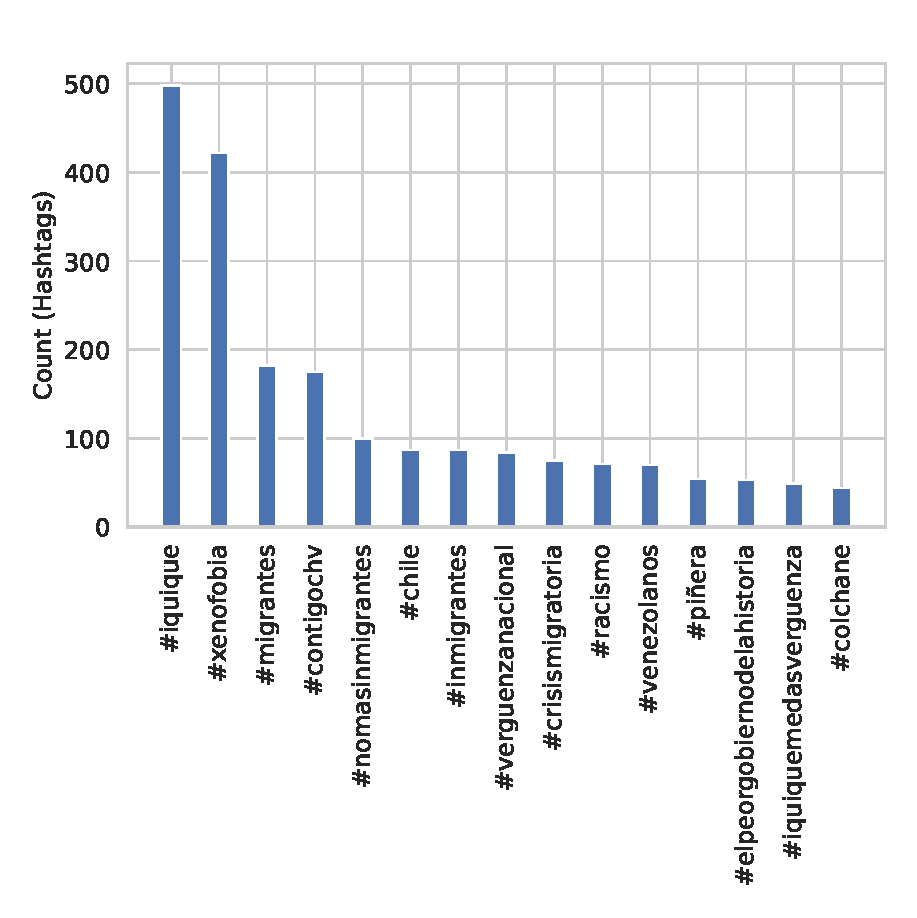
\includegraphics[width=.99\linewidth]{figs/Left_Hashtags_Protest_1.eps}
                \label{fig_hashtags_protest_lef}
            \end{subfigure}%
        %\hfill
            \begin{subfigure}{0.5\textwidth}
                \caption{Right-Leaning Twitter Users}
                \centering
                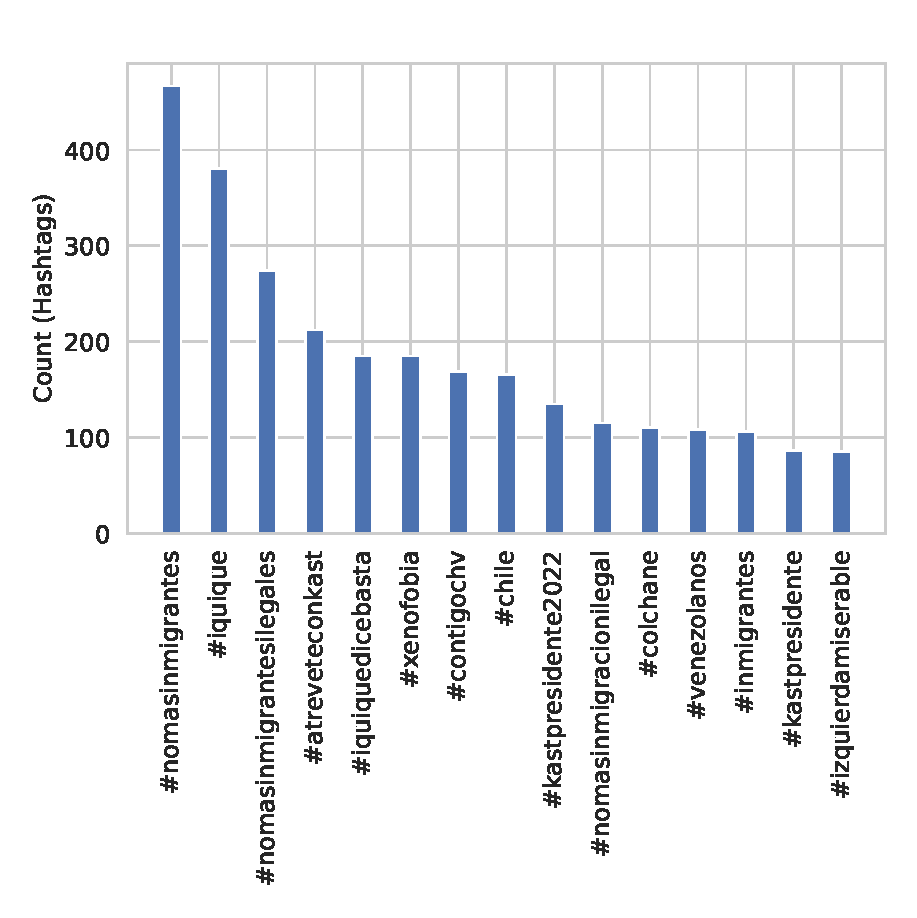
\includegraphics[width=.99\linewidth]{figs/Right_Hashtags_Protest.eps}
                \label{fig_hashtags_protest_rig}
            \end{subfigure}
        \hfill
            \begin{subfigure}{0.5\textwidth}
                \caption{Unlabeled Twitter Users}
                \centering
                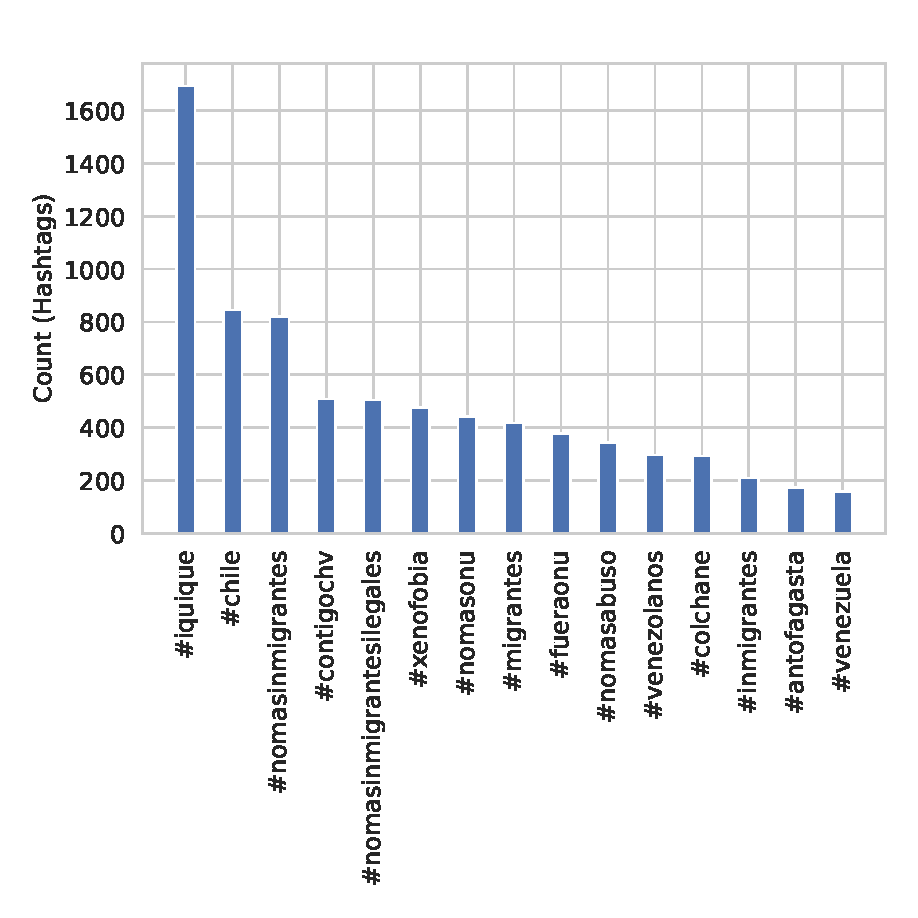
\includegraphics[width=.99\linewidth]{figs/Unlabeled_Hashtags_Protest_1.eps}
                \label{fig_hashtags_protest_unlab}
            \end{subfigure}
        
    \floatfoot{\it 
                Notes:  Textual preprocessing steps in outputs include lowercase enforcement and converting Spanish special characters (e.g. á, ñ, etc.) into corresponding non-accentuated ones.
                \vspace{0.5em} \\
                Data Source: Subsample of main corpus retrieved from Twitter API, 5 days before and after the protest, i.e. Sep 21, 2021 to Oct 1, 2021. Affiliation labels constructed using Step 6 in our methodology as described in Section \ref{sec_meth_gene} and Appendix \ref{app_sec_meth}. Corpus includes tweets by Twitter users in Chile or Chilean nationals that mainly pertain to immigration.}
    \end{figure}
    
        \newline\indent
    
    
    %show how often each hashtag or bigram was used and how many users include it in their tweets for each of the previous figures.
    
    %Figures \ref{fig_bigram_protest_unlab} and \ref{fig_hashtags_protest_unlab} show the most frequent bigrams and hashtags for unlabeled users, respectively. These give indications towards the ideological affiliations of unlabeled users as discussed further in Section \ref{unlab_users_affiliation}. However, there are some common bigrams for unlabeled users that neither left-leaning nor right-leaning users use. This is specifically the mention of the UN ({\it 'ONU'} in Spanish). In Figure \ref{fig_bigram_protest_unlab} the mention of \texttt{@onuchile} is prevalent, while Figure \ref{fig_hashtags_protest_unlab} shows that hashtags such as \texttt{\#fueraonu} (Eng: Out with the UN) and \texttt{\#nomasonu} (Eng: No more UN) are popular among unlabeled Twitter users. Reviewing how many users include these hashtags or bigrams, we can see that there are only a few of them that tweet a lot. Again, we find that something that appears to be a general pattern in truth is a little group of people trying to push some topic in the discussion.
        

    %Figure \ref{fig_bigram_protest_unlab} might also give us some insights as to which ideology is most prevalent in the 'Unlabeled' category. The distribution of bigrams is more akin to that of the right-leaning users and so are the connotations of the bigrams. We find unlabeled users to mainly stress the undocumented/illegal situation of the migrants with popular bigrams such as {\it 'inmigrantes, ilegales'} (Eng: Immigrants, illegals), {\it 'crisis, migratoria'} (Eng: Crisis, migratory), {\it 'marcha, encontra'} (Eng: March, against) and {\it 'encontra, migrantes'} (Eng: Against, migrants). So in the unlabeled category we find that these are more similar to right-leaning users. Either we have some right-leaning users in the 'Unlabeled' category that our labeling strategy classifies wrongly. It could also be the case that unlabeled users are in fact center-leaning and that center voters are more anti-immigration than embracing. 
    
    %However, one finding points towards that the 'Unlabeled' category mainly includes individuals with similar opinions than right-leaning users .  For unlabeled users we find that they use hashtags such as \texttt{\#nomasinmigrantes} (Eng: No more immgirants) and \texttt{\#nomasinmigrantesilegales} (Eng: No more illegal immigrants) which mainly mirror the talking points of the right.However, there are some common bigrams for unlabeled users that neither left-leaning nor right-leaning users use. This is specifically the mention of the UN ({\it 'ONU'} in Spanish). In Figure \ref{fig_bigram_protest_unlab} the mention of \texttt{@onuchile} is prevalent, while Figure \ref{fig_hashtags_protest_unlab} shows that hashtags such as \texttt{\#fueraonu} (Eng: Out with the UN) and \texttt{\#nomasonu} (Eng: No more UN) are popular among unlabeled Twitter users. These bigrams and hashtags show that people blame the UN for the uncontrolled immigration. %However, we find one specific talking point from the right-leaning individuals which is \texttt{\#xenofobia} (Eng: Xenophobia). With these findings in mind, we cannot claim that unlabeled users primarily are right-leaning as the use of hashtags is ambiguous across ideological agendas. However, unlabeled users are primarily reminiscent of the right-leaning users and if we assume anti-UN sentiments to be right-wing agendas, it could be a reasonable assumption that unlabeled users are primarily right-leaning. In this case the findings from Figure \ref{fig_terms} could potentially be even starker.

    
    
%\vspace{5em}
    
    %Looking at the results, we can see that the main emphasis of right-leaning users is the illegal immigration. The two most common bigrams (and far away the others) are related with the word {\it 'illegal'}. Also, looking at the following bigrams, other topics appear as relevant. One of them is the interpolation to some institutions ({\it 'Congreso'} and {\it 'CC'} that means Constitutional Convention) and the link with the Venzuelan dictatorship Nicolás Maduro. On the other hand, for left-leaning users the word {\it 'illegal'} does not appear in the common bigrams. They put the focus on the migratory flux ({\it '(venir, chile)'} for instance), in the burned stuff ({\it 'pertenencias'}, {\it 'coches'}, {\it 'pañales'}) in xenophobia and racism  and also they relate the event with a previous visit of the president Piñera to Venezuela ({\it '(Piñera, Cúcuta)'}).

    %Finally, an interesting finding appears looking at the most common bigrams for unlabeled users. First, the two most common hashtags coincide with right-leaning people emphasizing the word illegal, but after that appear a new topic that does not appear both for neither right- nor left-leaning Twitter users. This is the mention of the UN ({\it 'ONU'} in Spanish) and the link that these people make between immigration, the protest and the UN agenda. The bigrams show that people blame the UN for the uncontrolled immigration.
    
    %If we want to go deeper in the analysis, we can look at the most common hashtags for each political affiliation, to see if they are consistent with the things that bigrams show.
    
    
    
    
    
    
    %KALL:
    

    
    
    %Here appears some information that confirms our previous findings, e.g. the most common hashtag used by the right-leaning people is against the immigration or like the hashtag against UN appears only for unlabeled people. But new insights appear. For instance, we can see that right-leaning people link the immigration issue during this week with the electoral campaign, using different hashtags to promote their candidate. In the left-wing this does not happen. On the other hand, left-leaning people used some hashtags to blame the government for the situation. Also, in the three graphs appear the hashtag \texttt{\#contigochv}, which is related to a morning TV show. This also shows a TV program that was generating discussion about the topic and is generating transversally to the political spectrum.